
\newcommand{\hc}{h_\text{c}}
\newcommand{\hf}{h_\text{f}}

\newcommand{\sigmafail}{\sigma_\text{y}}
\newcommand{\sigmafailz}{\sigma_\text{yZ}}
\newcommand{\taufail}{\tau_\text{y}}
\newcommand{\tauz}{\tau_\text{yZ}}

\begin{figure}[H]
	\centering
	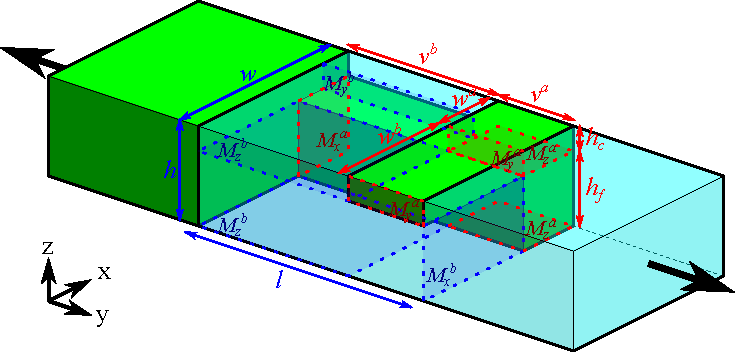
\includegraphics[width=\columnwidth]{sources/method/straight_model_v3.pdf}
	\caption{
		One straight unit cell connecting material $a$ (left) to material $b$ (right).
		Failure can happen along the fingers ($M_x$), along the cross beams ($M_y$) or at the interface between the two ($M_z$) for either material.}
	\label{fig:failure_modes}
\end{figure}


\section{Straight design}

\iffalse
The bending constraint is given by:
\begin{align*}
	\sigma_\text{max} &= \frac{M}{I}c \\
	c &= \nicefrac12 h \\
	I &= \frac{b h^3}{12} \\
	M &= \frac{w L^2}{12} \\
	w &= \frac{F}{L} \\
	\sigma_\text{max} &= \frac{w L^2 / 12}{b h^3 / 12} \nicefrac12 h \\
	\sigma_\text{max} &= \frac{w L^2}{b h^3} \nicefrac12 h \\
	\sigma_\text{max} &= \frac{F L}{b h^3} \nicefrac12 h \\
	\sigma_\text{max} &= \frac{F L}{2 b h^2} \\
\end{align*}
\fi


\Cref{fig:failure_modes} shows one cell of the straight structure, along with the design variables and the failure modes.
We want to optimize the effective ultimate tensile strength, while keeping the structure minimal.
Below you will find a naive formulation of the optimization problem.
The naive model will be fine-tuned and several variants will be considered.
Finally we compare the variants against experimental FEM simulation results in order to get to the final formulation of the optimization problem.
\footnote{Even though finding the correct model is not the focus of this course, it is relevant to my PhD research and we cover several interesting ideas pertaining to engineering optimization.}
The naive problem formulation is as follows:

\begin{align}
	& \omit\rlap{$\displaystyle \max{ \frac{F}{\left( w^a + w^b \right) \left( \hf + \hc \right) }}$} \label{eq:obj} \\
	& \omit\rlap{$\displaystyle \min{ \hf + \hc} $} \nonumber \\
	& \omit\rlap{$\displaystyle \min{ w^a + w^b} $} \nonumber \\
	\omit\rlap{subject to} \nonumber \\
	w^m &\ge 2 \wmin^m			&&\text{ Nozzle size} \label{eq:c1} \\
	v^m &\ge \wmin^m				&&\text{ Nozzle size}  \label{eq:c2} \\
	\hf &\ge \hmin		&&\text{ Layer thickness}  \label{eq:c3} \\
	\hc &\ge \hmin		&&\text{ Layer thickness}  \label{eq:c4} \\
	v^a + v^b &\le \lmax         &&\text{ Design constraint}   \label{eq:c_total_length} \\
	\sigma_{11}^m = \frac{ F }{ w^m \hf } &\le \sigmafail^m					&&\text{ Tension failure } M_x^m  \label{eq:c_tensile} \\
	\sigma_{13}^m = \frac{ F w^{\neg m} }{ 2 v^m \hc w } &\le \taufail^m					&&\text{ Shear failure } M_y^m  \label{eq:c_shear} \\
	\sigma_{22}^m = \frac{ F \left(w^{\neg m}\right)^2 }{ 2 \left( v^m \right)^2 \hc w } &\le \sigmafail^a                 &&\text{ Bending failure } M_y^m  \label{eq:c_bending} \\
	\sigma_{12}^m = \frac{ F }{ 2 v^m w^m} &\le \tauz^m							&&\text{ Shear failure } M_z^m  \label{eq:c_shear_z} \\
	\omit\rlap{for both materials $m \in \{a, b\}$ where $\neg a = b$ and $\neg b = a$}\nonumber
\end{align}

The first objective function is the main objective; 
the other two objective functions are secondary.
They are only introduced to disambiguate designs which have the same value for the objective function --
that is: pareto optimality is introduced to disambiguate otherwise equivalent designs.

Note that the $v^m$ variables don't figure in the objective,
but they do appear in the constraints and therefore are also subject to the optimization.
Some of the mechanical constraints will be active to provide them a definite value.

\subsection{Stress formulae}
Let's consider the stresses $\sigma$ induced by applying a force to the ends of the unit cell.
Tensile stress in the finger of either material $m$ is given by:
\begin{align*}
	\sigma_{11}^m &= \frac{ F }{ w^m \hf }
\end{align*}

The shear stress acting on $M_y^m$ for either material $m$ is determined by modeling the unsupported portion of the cross beam as a doubly fixed beam,
whereas the total load is modeled as being uniformly distributed over the whole beam.
The portion $d_y^m$ of the total force $F$ which acts upon the unsupported part of material $a$ is proportional to $w^b / w$, where $w = w^a+w^b$.
However, in some cases the full force acts on the beam, which will be discussed below.
To select between these cases we can switch the $u_y^m$ parameter between zero and one.
Because the beam is fixed on both sides the shear force is half the total force acting on the beam.
\begin{align*}
	\sigma_{13}^m &= \frac{d_y^m F}{2 v^m \hc} \\
	d_y^m &= \frac{w^{\neg m} + u_y^m w^m}{w}
\end{align*}


The same unsupported portion of the cross beam might be subject to bending.
The highest bending stress for a doubly supported beam will occur on either end.
\begin{align*}
	\sigma_{22}^m &= \frac{M}{I}c = \frac{d_y^m F w^{\neg m} / 12}{\hc (v^m)^3 / 12} \nicefrac12 v^m 
	=  \frac{ d_y^m F w^{\neg m} }{ 2 \left( v^m \right)^2 \hc }
	= \sigma_{13}^m \frac{w^{\neg m}}{v^m}
\end{align*}

There is also a shear stress acting along the surface $M_z^m$.
On the one hand one might think that only a portion $d_z^m$ of the total force $F$ is working on the supported portion of the cross beam.
On the other hand the total force must be enacted through this plane, because it is the only connection between the finger and the cross beam.
The term $u_z^m$ switches between fractional and full force by setting it to zero or one respectively.
In order to compare stresses along the Z direction and stresses along the XY direction against the same ultimate stress value $\sigmafail$,
we multiply the Z shear stress by the ratio $\nicefrac{\sigmafail}{\sigmafailz}$.
The shear stress along Z is therefore given by:
\begin{align*}
	\sigma_{12}^m &= \frac{\sigmafail}{\sigmafailz} \frac{ d_z^m F }{ 2 v^m w^m} \\ 
	d_z^m &= \frac{w^m + u_z^m w^{\neg m}}{w}
\end{align*}



\subsection{Constraint values}
Under different circumstances the values of the constraints will be different.
Different nozzles and different layer thickness settings require different constraint values.
Because of manufacturing constraints we know that the layer thickness has to be smaller than half the smallest nozzle size:
$\hmin < \nicefrac{1}{2} \wmin^m$.

Materials properties of 3D printed materials are always such that $\tauz^m < \taufail^m$.
According to the von Mises yield criterion we have that $\taufail^m = \sigmafail^m / \sqrt{3} $.

Depending on the types of material used the tensile and shear strength in the Z direction can be an order of magnitude lower than in the horizontal directions.
In such a case the Z shearing failure constraints \cref{eq:c_shear_z} will be active for that material.

Depending on the design we might apply a different $\lmax$, 
but it is required that $\lmax \ge \wmin^a + \wmin^b$.

\subsection{Boundedness}
The manufacturing constraints provide sufficient lower bounds, but the upper bounds are problematic in the current formulation.
The design constraint effectively places an upper bound on the $v^m$ widths.
One might think that this constraint drives the other design variables to some finite value as well.
However, in this section we show how the current formulation will be amended to make the problem well-behaved.

\label{sec:domain_assumptions}
If we would scale all design variables linearly with some factor $R$ and $F$ by $R^2$ then the objective function and all mechanical constraints \crefrange{eq:c_tensile}{eq:c_shear_z} remain at the same value.
If only those constraints were to be considered the problem would have been under-constrained.
Since one of our objective functions is to minimize the total width $(w^a + w^B)$ we know that some of the constraints \crefrange{eq:c1}{eq:c4} will have to be active.
If we set \cref{eq:c1} active for material $a$ we will show that none of the other constraints will be violated, so this constraint has to be active.

The same holds for the heights.
We can scale $\hc$, $\hf$ and $F$ down with a factor $R$ without changing the value of the objective function nor the mechanical constraints \crefrange{eq:c_tensile}{eq:c_bending}.
The Z shear constraint \cref{eq:c_shear_z} does change, but as long as we scale down $R<1$ this constraint will remain satisfied.
This means the problem definition is not well-defined.
In order to solve this we use the height objective function $(\hf + \hc)$ to set \cref{eq:c4} active and we will show that \cref{eq:c3} is not violated.


\subsection{Constraint redundancy}
If $\nicefrac{w^b}{v^a} > \nicefrac{ \sigmafail^a }{ \taufail^a } = \sqrt{3}$ 
then the shear failure constraints \cref{eq:c_shear} for material $a$ is dominated by the bending failure constraint \cref{eq:c_bending},
since then 
$
\frac{ d_y^m F w^b }{ 2 \left( v^a \right)^2 \hc \sigmafail^a}
> \frac{ d_y^m F }{ 2 v^a \hc \taufail^a} 
$.
Otherwise the latter is dominated by the former.
The same holds conversely with the materials $a$ and $b$ swapped.
Therefore two of \cref{eq:c_shear,eq:c_bending,eq:c_bending} will be redundant.
We could combine those four constraints into two single ones:
\begin{align}
	%\frac{ d_y^m F }{ 2 v^m \hc} &\le \taufail^m \\
	%\frac{ d_y^m F }{ 2 v^m \hc} &\le \nicefrac1{\sqrt{3}} \sigmafail^m \\
	%\frac{ d_y^m F }{ 2 \cdot \sqrt{3} v^m \hc} &\le \sigmafail^m \\
	%???\frac{ d_y^m F w^b }{ 2 \left( v^a \right)^2 \hc } &\le \sigmafail^a \\
	%\\
	\frac{ d_y^m F }{ 2 v^a \hc }  \max{\left( \sqrt{3}, \frac{w^b}{ v^a} \right)} &\le \sigmafail^a  \nonumber \\
	\frac{ d_y^m F }{ 2 v^b \hc }  \max{\left( \sqrt{3}, \frac{w^a}{ v^b} \right)} &\le \sigmafail^b  \label{eq:shear_bend_combined}
\end{align}


\subsection{Von Mises criterion}
However, when these criteria are near-active then there could be an interaction between the two.
The shear and bending interact and thereby lower the force at which failure happens.
In order to estimate the combined failure criterion we consider the von Mises yield criterion:

\begin{align*}
	\left(\sigma_{11} - \sigma_{22}\right)^2  +  \left(\sigma_{22} - \sigma_{33}\right)^2  +  \left(\sigma_{33} - \sigma_{11}\right)^2  \\
	+   6\left(\sigma_{23}^2 + \sigma_{13}^2 + \sigma_{12}^2\right) &< 2 \sigmafail^2 \\
\end{align*}

Using the von Mises criterion to combine the shear stress $\sigma_{13}$ and the bending stress $\sigma_{22}$, we get:

\begin{align}
	% \sqrt{ \left(  \frac{ d_y^m F w^b }{ 2 \left( v^a \right)^2 \hc }  \right)^2   +   3 \left(  \frac{ d_y^m F }{ 2 v^a \hc}  \right)^2 } &< \sigmafail^a \\
	% \sqrt{ \left(  \frac{ d_y^m F }{ 2 v^a \hc} \frac{w^b}{v^a}  \right)^2   +   3 \left(  \frac{ d_y^m F }{ 2 v^a \hc}  \right)^2 } &< \sigmafail^a \\
	% \sqrt{ \left(  \frac{ d_y^m F }{ 2 v^a \hc}\right)^2  \left( \frac{w^b}{v^a}  \right)^2   +   3 \left(  \frac{ d_y^m F }{ 2 v^a \hc}  \right)^2 } &< \sigmafail^a \\
	% \sqrt{ \left(  \frac{ d_y^m F }{ 2 v^a \hc}\right)^2  \left( \left( \frac{w^b}{v^a}  \right)^2   +   3  \right) } &< \sigmafail^a \\
	\sigma_{13,22}^a = \frac{ d_y^m F }{ 2 v^a \hc} \sqrt{   \left( \frac{w^b}{v^a}  \right)^2 + 3 } &< \sigmafail^a \nonumber \\
	\sigma_{13,22}^b = \frac{ d_y^m F }{ 2 v^b \hc} \sqrt{   \left( \frac{w^a}{v^b}  \right)^2 + 3 } &< \sigmafail^b \label{eq:shear_bend_von_mises}
\end{align}

Note that the von Mises yield criterion \cref{eq:shear_bend_von_mises} is de facto equivalent to the application of the P-norm smooth approximation of the maximum function as used in the combined constraint \cref{eq:shear_bend_combined}, for $P=2$.
What a neat coincidence!
Where $\nicefrac{w^b}{v^a} \to 0$ and $\nicefrac{w^b}{v^a} \to \infty$ the failure is dominated by shear and bending respectively. 
This shows that in the limits the von Mises yield criterion and the combined criterion coincide.

We can similarly postulate combined von Mises constraints for tensile failure $M_x$ and Z shear failure $M_z$: $\sigma_{11,12}$.
And also for Z shear failure $M_z$ and cross beam failure $M_y$, including bending: $\sigma_{12,13,22}$; or without: $\sigma_{12,13}$.
One might even consider a combined con Mises constraint for all stresses together: $\sigma_{11,12,13,22}$.


\subsection{Constraint validity}
A careful analysis of the geometry will show that once shearing failure mode $M_x^a$ has occurred, 
there is still interlocking between the two materials;
once part of the cross beams of $b$ has sheared off, still a column of material $a$ remains, which is surrounded by material $b$.
Once one of those failure modes has occurred still any other failure mode has to occur for the interlock to fail, except $M_x^b$.
The only constraint added by the shearing failure modes should therefore be that both those failure modes occur together.
The constraint is violated only when both occur, so it is satisfied when either failure mode is prevented.
The logical disjunction can be rewritten into a minimum when both constraints are transformed into negative null form:
\begin{align*}
	% \min \left(  \frac{ d_y^m F }{ 2 v^a \hc \sigmafail^a} \sqrt{   \left( \frac{w^b}{v^a}  \right)^2 + 3 }  ,  \frac{ F }{ 2 v^b \hc \sigmafail^b} \sqrt{   \left( \frac{w^a}{v^b}  \right)^2 + 3 }  \right) - 1 &< 0 \\
	% \frac{ d_y^m F }{ 2 \hc}  \min \left(  \frac{ 1 }{ v^a \sigmafail^a} \sqrt{   \left( \frac{w^b}{v^a}  \right)^2 + 3 }  ,  \frac{ 1 }{ v^b \sigmafail^b} \sqrt{   \left( \frac{w^a}{v^b}  \right)^2 + 3 }  \right) - 1 &< 0 \\
	\frac{ d_y^m F }{ 2 \hc}  \min \left(  \frac{ \sqrt{   \left( \frac{w^b}{v^a}  \right)^2 + 3 } }{ v^a \sigmafail^a}   ,  \frac{  \sqrt{   \left( \frac{w^a}{v^b}  \right)^2 + 3 } }{ v^b \sigmafail^b}  \right) - 1 &< 0 \\
	% \frac{ d_y^m F }{ 2 \hc}  \min \left(  \frac{ \sqrt{   \left(w^b\right)^2 + 3 \left(v^a\right)^2 } }{ \left(v^a\right)^2 \sigmafail^a}   ,  \frac{  \sqrt{   \left(w^a\right)^2 + 3 \left(v^b\right)^2 } }{ \left(v^b\right)^2 \sigmafail^b}  \right) - 1 &< 0 \\
\end{align*}

Depending on the optimization algorithm used, the min operator might need to be replaced by smooth versions.
The choice between P-norm, Kreisselmeier-Steinhauser function or any of the other alternatives might be decided by properties of their derivatives.
The height of the $P$ value will determine the approximation error.
The approximation error of the max function means that the approximated constraint is more strict than the underlying sub-constraints, 
while the smooth approximation of the min function is more lenient.
This means that using a smooth approximation of this constraint could result in infeasible designs according to the analytical constraint.

Because the elongation at failure for PP is much higher than for TPLA, we expect that in case both cross-beams break the PLA one will break before the PP one.
We can therefore consider the situation where the cross beam shear constraint of material $a$ is violated and optimize the structure while adhering to the cross beam shear constraint of material $b$.
See \cref{fig:straight_model_broken}.
In this situation the cross beam shear and bending constraints for material $a$ don't hold.
Note that in the broken configuration the total force cannot be uniformly distributed over the whole length $w$, so we specify:
$
	u_y^a = \text{N/A};
	u_y^b = 1 ;
	u_z^a = 1 ;
	u_z^b = 1
$.

\begin{figure}[H]
	\centering
	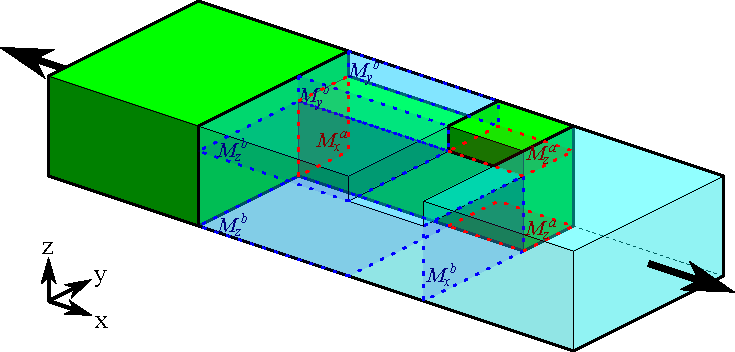
\includegraphics[width=\columnwidth]{sources/method/straight_model_v3_broken.pdf}
	\caption{The straight model when part of the cross beam has sheared off at $M_y^a$.}
	\label{fig:straight_model_broken}
\end{figure}

Including that in a single constraint is not an easy task, however.
One might combine all constraints containing the term $d_y^m$ into a single constraint.
Better yet - one might combine all constraints into a single one using the following scheme:
\begin{align*}
	\begin{array}{l}
		h_1(\mathbf{x}) < 0 \\
		\vdots \\
		h_N(\mathbf{x}) < 0 \\
	\end{array}
	\to
	\max \left(h_1(\mathbf{x}), \dots, h_N(\mathbf{x}) \right) < 0
\end{align*}
Using a smooth version of the $\max$ function like described above can overcome undifferentiability issues.
However, combining all constraints into a single one hinders analysis and understanding of a particular datum in the design space.


%\todo{TODO: rescale objective function so that they are approximately in the range 0-1.}

%\todo{TODO: should we invert the mechanical constraints, so that the F is below the division line?}



\subsection{Model evaluation}
When subjecting the microstructure to a load the distribution of stress is difficult to predict, because of the interplay between several failure modes.
Our model makes some strong assumptions on the homogeneity of stress distribution throughout the beams.
We mentioned several modeling choices which were deferred: the values for $u^m_y$, $u^m_z$, the exclusion of the bending constraints and using combined von Mises criterions.
In order to evaluate which of the variants of our analytical model is best we compare against an extensive grid search of FEM simulations.
\footnote{The FEM simulations were not performed by either of the two students. The implementation details of the FEM simulation are left out of this report.}

The simluations were performed on a grid along three dimensions: $w^b$, $v^a$ and $\hf$, within the ranges $(0.6,3.0)$, $(0.1\lmax, 0.9\lmax)$ and $(1.8, 3.6)$ respectively.
Because the design constraint is active, and because the minimum feature size is active, we can derive $w^a$, $v^b$ and $\hc$ from these.
The output of each simulation is a force $F$, which can be used to compute the ultimate tensile strength $f$ of a given design.

Similarly we converted our problem such that for each design in the 3D space, we compute the force according to each mechanical constraint.
For example, the minmum force according to the tensile constraint for $a$ would be $F = \sigmafail^a w^a \hf$.
Because the structure will fail as soon as the first mechanical constraint is violated,
we record the minimum force for all constraints and use that to compute the predicted ultimate strength.
Also for the comparison we set $\sigmafailz^m = \sigmafail^m$, because the FEM simulations cannot capture the difference in strength along the Z direction caused by the layerwise buildup of FDM 3D printing.

\begin{table}
	\centering
	\caption{Accuracy of the analytical model w.r.t. FEM results.}
	\label{tab:prediction_ratios}
	\begin{tabular}{llll|ll}
		$u^m_z$ & $\sigma_{22}$ & $\sigma_{11,12}$ & $\sigma_{12,13}$ & $\nicefrac{F}{\hat{F}}$ & std dev \\
		\hline
		\checkmark & - & - & - & 104.2\% & 19.8\% \\
		\checkmark & - & - & \checkmark & 101.7\% & 18.9\% \\
		\checkmark & - &\checkmark&\checkmark & 94.7\% & 19.3\% \\
		\checkmark & - &\checkmark& - & 97.0\% & 20.5\% \\
		\checkmark &\checkmark& - & - & 85.3\% & 31.0\% \\
		- & - & - &\checkmark& 107.6\% & 16.2\% \\
		- & - & - & - & 107.8\% & 16.2\% \\
	\end{tabular}
\end{table}

We compare each point in the FEM data set to our analytical model,
and calculate the average prediction ratio $\nicefrac{F}{\hat{F}}$ between the simulated $\hat{F}$ and the analytically predicte $F$, along with the standard deviation.
See \cref{tab:prediction_ratios}.
From these results we can see that including the bending stress $\sigma_{22}$ doesn't improve the accuracy of our analytical model.
Also the $\sigma_{11,12}$ von Mises criterion which combines tensile and Z shear lowers teh accuracy.
Using the $\sigma_{12,13}$ von Mises criterion to combine the stresses in the cross beam with the Z shear stress does improve the model.

The question whether we should use the full force for computing the Z shear stress $u^m_z$ is more difficult to answer;
while it gets the prediction ratio closer to \SI{100}{\percent}, the standard deviation increases.
It makes sense that the analytical model overestimates the ultimate strength, because we assume homogenous stress distributions.
Omitting $u^m_z$ may cause an increase in prediction ratio, but the overall shape is closer o the FEM predictions as indicated by the lower standard deviation.
Because we are less concerned with the actual ultimate strength, and more in the optimal design, we will choose to only use the partial force when computing the Z shear stress.

The comparison on the final model is shown in \cref{fig:ana_vs_FEM}.
We can then reintroduce the correct value for $\sigmafailz^m$ and evaluate the analytical model on a more dense grid.
See \cref{fig:ana_minF}.
One important observation is that we can distinguish 4 constraint surfaces which culminate in the same optimum, while there are only 3 free design variables.
The fact that 4 surfaces meet in a 3-dimensional space is not to be thought of as a coincidence, but is presumably inherent to the particular problem at hand.

When evaluating the converted analytical model,
we can easily verify that all domain constraints are met,
so we were justified in assuming the value for $w^a$ and $\hc$ in \cref{sec:domain_assumptions}.
That is to say: since none of the other design variables are below thair lower bound it was safe to assume that it were these two variables which had to be at their lower bound rather than any of the others.


\begin{figure}
	\centering
	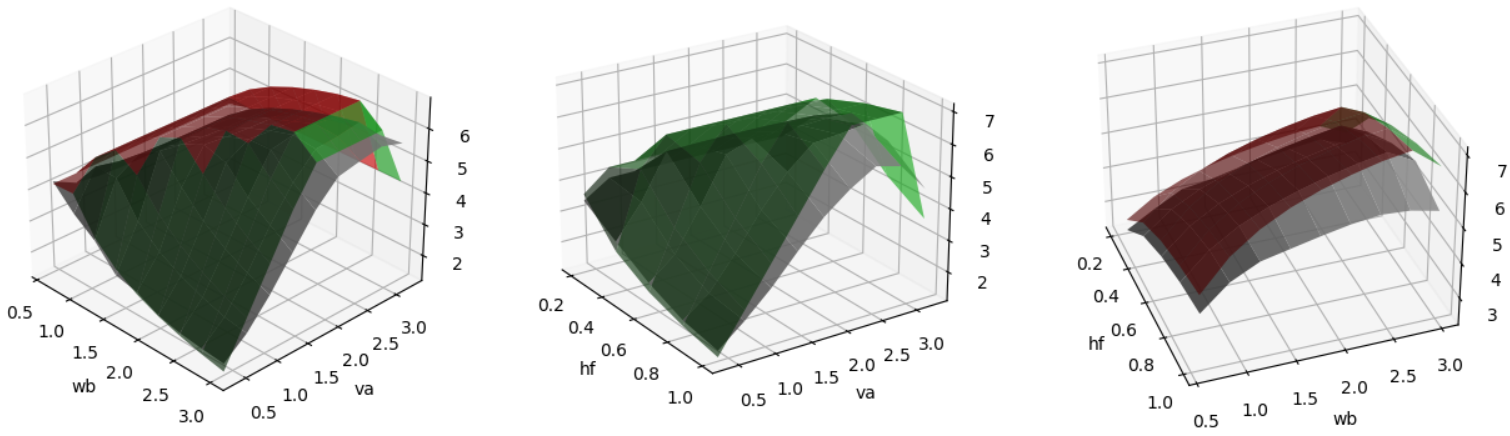
\includegraphics[width=\columnwidth]{sources/method/ana_vs_FEM.png}
	\caption{Ultimate tensile strength, colored according to failure mode and FEM simulation results in gray.
	These are three 2D slices through the 3D space spanned by $w^b$, $v^a$ and $\hf$, sliced at the maximum ultimate strength value.
	}
	\label{fig:ana_vs_FEM}
\end{figure}



\begin{figure}
	\centering
	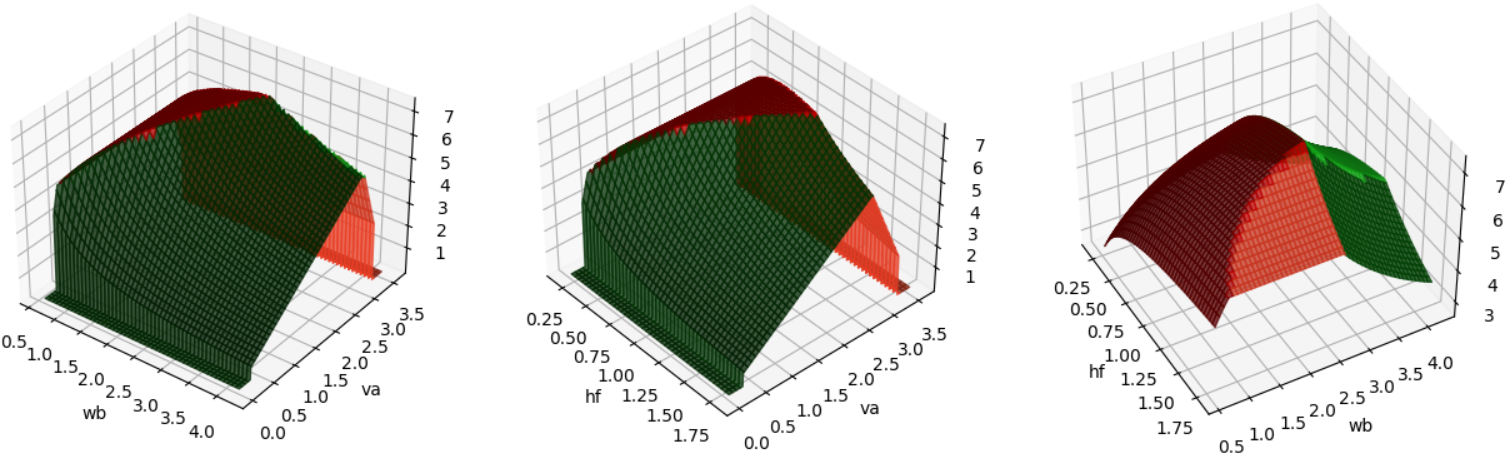
\includegraphics[width=\columnwidth]{sources/method/ana_minF.png}
	\caption{Ultimate tensile strength, colored according to failure mode according to the validated model.
	These are three 2D slices through the 3D space spanned by $w^b$, $v^a$ and $\hf$, sliced at the maximum ultimate strength value.
	}
	\label{fig:ana_minF}
\end{figure}



\subsection{Problem reformulation}
Taking the above into account we reformulate the problem.
The shear constraints are combined into one.
The constraints which hold for both materials are expanded.
The variables set by the presumed to be active constraints are substituted.
To our regret the design variables have not been scaled so as to all lie approximately in the domain $(0,1)$.

We divide by the constraint values and invert the division of the mechanical constraints.
That way the formulae of those constraints are more alike and simpler to differentiate.

% shear + Z shear constraint derivation
\iffalse
\begin{align*}
	%2 ( \sigma_{12,13} )^2 &= \\
	%6\left(\sigma_{13}^2 + \sigma_{12}^2\right) &< 2 \sigmafail^2 \\
	%3\left(\sigma_{13}^2 + \sigma_{12}^2\right) &< \sigmafail^2 \\
	%\sigma_{12,13} =
	\sqrt{ 3\left(\sigma_{13}^2 + \sigma_{12}^2\right) }  &< \sigmafail \\
	\frac{\sigmafail}{\sqrt{ 3\left(\sigma_{13}^2 + \sigma_{12}^2\right) }} &> 1 \\
	1 - \frac{\sigmafail}{\sqrt{ 3\left(\sigma_{13}^2 + \sigma_{12}^2\right) }} &< 0 \\
	1 - \frac{\sigmafail}{\sqrt{ 3\left( \left( \frac{d_y^m F}{2 v^m \hc} \right)^2 + \left(  \frac{\sigmafail}{\sigmafailz} \frac{ d_z^m F }{ 2 v^m w^m}  \right)^2\right) }} &< 0 \\
	3\left( \left( \frac{d_y^m F}{2 v^m \hc} \right)^2 + \left(  \frac{\sigmafail}{\sigmafailz} \frac{ d_z^m F }{ 2 v^m w^m}  \right)^2\right) &< \sigmafail^2\\
	3\left( \left( \frac{d_y^m F}{2 v^m \hc} \right)^2 + \left(  \frac{\sigmafail}{\sigmafailz} \frac{ w^m F }{ 2 v^m w^m w}  \right)^2\right) &< \sigmafail^2\\
	3\left( \left( \frac{d_y^m F}{2 v^m \hc} \right)^2 + \left(  \frac{\sigmafail}{\sigmafailz} \frac{ F }{ 2 v^m w}  \right)^2\right) &< \sigmafail^2\\
	3\left(\frac{F}{2v^m}\right)^2 \left( \left( \frac{d_y^m }{\hc} \right)^2 + \left(  \frac{\sigmafail}{\sigmafailz} \frac{ 1 }{ w}  \right)^2\right) &< \sigmafail^2\\
	\sqrt{3} \frac{F}{2v^m} \sqrt{ \left( \frac{d_y^m }{\hc} \right)^2 + \left(  \frac{\sigmafail}{\sigmafailz w} \right)^2 } &< \sigmafail\\
	\sqrt{3} \frac{F}{2v^m} \sqrt{ \left( \frac{1 }{\hc} \frac{w^{\neg m}}{w} \right)^2 + \left(  \frac{\sigmafail}{\sigmafailz w} \right)^2 } &< \sigmafail\\
	\sqrt{3} \frac{F}{2v^m} \sqrt{ \left( \frac{w^{\neg m}}{w \hc} \right)^2 + \left(  \frac{\sigmafail}{\sigmafailz w} \right)^2 } &< \sigmafail\\
	\sqrt{3} \frac{F}{2v^m w} \sqrt{ \left( \frac{w^{\neg m}}{ \hc} \right)^2 + \left(  \frac{\sigmafail}{\sigmafailz} \right)^2 } &< \sigmafail\\
	\frac{2v^m w}{F} \frac{1}{ \sqrt{3} \sqrt{ \left( \frac{w^{\neg m}}{ \hc} \right)^2 + \left(  \frac{\sigmafail}{\sigmafailz} \right)^2 } } &> \frac{1}{\sigmafail}\\
	\frac{2v^m w}{F} \frac{\sigmafail}{ \sqrt{3} \sqrt{ \left( \frac{w^{\neg m}}{ \hc} \right)^2 + \left(  \frac{\sigmafail}{\sigmafailz} \right)^2 } } &> 1 \\
	1 - \frac{2v^m w}{F} \frac{\sigmafail}{ \sqrt{3} \sqrt{ \left( \frac{w^{\neg m}}{\hc} \right)^2 + \left(  \frac{\sigmafail}{\sigmafailz} \right)^2 } } &< 0 \\
	1 - \frac{2v^m w}{F} \frac{\sigmafail}{ \sqrt{ 3\left( \frac{w^{\neg m}}{ \hc} \right)^2 + 3\left(  \frac{\sigmafail}{\sigmafailz} \right)^2 } } &< 0 \\
	1 - \frac{2v^m w \sigmafail}{ F \sqrt{ 3\left( \frac{w^{\neg m}}{ \hc} \right)^2 + 3\left(  \frac{\sigmafail}{\sigmafailz} \right)^2 } } &< 0 \\
	%\\
	1 - \frac{2v^a w \sigmafail^a}{ F \sqrt{ 3\left( \frac{w^b}{ \hc} \right)^2 + 3\left(  \frac{\sigmafail^a}{\sigmafailz^a} \right)^2 } } &< 0 \\
	1 - \frac{2v^b w \sigmafail^b}{ F \sqrt{ 3\left( \frac{w^a}{ \hc} \right)^2 + 3\left(  \frac{\sigmafail^b}{\sigmafailz^b} \right)^2 } } &< 0 \\
\end{align*}
\fi


\newcommand{\gwb}{g_\text{wb}}
\newcommand{\gva}{g_\text{va}}
\newcommand{\gvb}{g_\text{vb}}
\newcommand{\ghf}{g_\text{hf}}
\newcommand{\gd}{g_\text{d}}
\newcommand{\gta}{g_\text{ta}}
\newcommand{\gtb}{g_\text{tb}}
\newcommand{\gca}{g_\text{ca}}
\newcommand{\gzb}{g_\text{zb}}


\begin{align*}
	f: & \min{ \frac{\left( 2 \wmin^a + w^b \right) \left( \hf + \hmin \right) }{F} }\\
	\gwb: & 1 - \nicefrac{w^b }{2 \wmin^b} \le 0 \\
	\gva: & 1 - \nicefrac{v^a }{\wmin^a} \le 0 \\
	\gvb: & 1 - \nicefrac{v^b }{\wmin^b} \le 0 \\
	\ghf: & 1 - \nicefrac{\hf}{\hmin} \le 0 \\
	\gd: & \frac{v^a + v^b}{ \lmax }  - 1 \le 0 \\
	\gta: & 1 - \frac{ 2 \wmin^a \hf \sigmafail^a }{ F } \le 0 \\
	\gtb: & 1 - \frac{ w^b \hf \sigmafail^b }{ F } \le 0 \\
	\gca: & 1 - \frac{2v^a (2\wmin^a + w^b) \sigmafail^a}{ F \sqrt{ 3\left( \frac{w^b}{ \hc} \right)^2 + 3\left(  \frac{\sigmafail^a}{\sigmafailz^a} \right)^2 } } \le 0 \\
	\gzb: & 1 - \frac{ 2 v^b w^b \tauz^b }{ F } \le 0
\end{align*}

\subsection{Monotonicity Analysis}
Below we show a monotonicity analysis.
The objective function is monotonically increasing in the width $w^b$ and height $\hf$, and monotonically decreasing in the force $F$.
Since none of the constraints are solely responsible for limiting a variable we are not able to reduce the problem definition further;
there are no critical constraints.

All mechanical constraints are conditionally critical for the design variables.

The non-objective variables $v^a$ and $v^b$ are bound by $\gva$, $\gvb$ and $\gd$.

\begin{align*}
	f: & F^-, w^{b+},  \hf^+\\
	%\omit\rlap{subject to} \nonumber \\
	\gwb: & w^{b-} \\
	\gva: & v^{a-} \\
	\gvb: & v^{b-} \\
	\ghf: & \hf^- \\
	\gd: & v^{a+}, v^{b+} \\
	\gta: & F^+, \hf^- \\
	\gtb: & F^+, w^{b-}, \hf^- \\
	\gca: & F^+, v^{a+}, w^{a+}, w^{b\pm} \\
	\gzb: & F^+, v^{b-}, w^{b-}
\end{align*}


\subsection{Monotonicity and Convexity}
Since the objective function doesn't contain any complex mathematical expressions one can easily see that it is monotonous.
All of the objective and constraint formulae are monotonous, but because of the the $F$ below the division line they are not convex.
We can therefore not preclude the existence of local optima.

If we would have used the disjunctive constraint on the cross beam failures, however, the feasible domain would definitely be non-convex.
The combined cross beam constraint entails the union of two feasible domains from the constraints relating to the two cross beams of the two materials.
Convexity is not invariant under union, so the convexity of the feasible space is not easily verified.
Given that the two sub-domains aren't dominated by the other, nor by any other constraint, we can derive that the disjunctive cross beam constraint would cause there to be at least two local minima in the design space.




\subsection{Sensitivity analysis}
The sensitivities are as follows:

\begin{align*}
	\frac{\partial f}{\partial v^a} &= \frac{\partial f}{\partial v^b} = 0 \\
	\frac{\partial f}{\partial w^b} &= \frac{\hf + \hmin}{F} \\
	\frac{\partial f}{\partial \hf} &= \frac{2 \wmin^a + w^b}{F} \\
	\frac{\partial f}{\partial F} &= - \frac{\left( 2 \wmin^a + w^b \right) \left( \hf + \hmin \right)}{F^2} \\
	\frac{\partial \log f}{\partial \log w^b} % &= \frac{\hf + \hmin}{F}  w^b \frac{F}{\left( 2 \wmin^a + w^b \right) \left( \hf + \hmin \right)} \\
	% &= \frac{\left( \hf + \hmin \right) w^b}{F} \frac{F}{\left( 2 \wmin^a + w^b \right) \left( \hf + \hmin \right)} \\
	% &= \frac{\left( \hf + \hmin \right) w^b}{\left( 2 \wmin^a + w^b \right) \left( \hf + \hmin \right)} \\
	&= \frac{ w^b }{ 2 \wmin^a + w^b} \\
	\frac{\partial \log f}{\partial \log \hf} % &= \frac{2 \wmin^a + w^b}{F} \hf \frac{F}{\left( 2 \wmin^a + w^b \right) \left( \hf + \hmin \right)} \\
	% &= \frac{\left(2 \wmin^a + w^b\right) \hf }{F} \frac{F}{\left( 2 \wmin^a + w^b \right) \left( \hf + \hmin \right)} \\
	% &= \frac{\left(2 \wmin^a + w^b\right) \hf }{\left( 2 \wmin^a + w^b \right) \left( \hf + \hmin \right)} \\
	&= \frac{ \hf }{ \hf + \hmin } \\
	\diff{\log{f}}{\log{F}} &= - 1 \\
\end{align*}

\iffalse
\begin{align*}
\begin{array}{c|ccccc} \nicefrac{\partial \_}{\partial \_} & w^b & v^a & v^b & \hf & F \\
    	\hline
	f & \frac{\hf + \hmin}{F}  & 0 & 0 & \frac{2 \wmin^a + w^b}{F} & - \frac{\left( 2 \wmin^a + w^b \right) \left( \hf + \hmin \right)}{F^2} \\
	\gwb & -\nicefrac{1}{2\wmin^b} & 0 & 0 & 0 & 0 \\
	\gva & 0 & -\nicefrac{1}{\wmin^a} & 0 & 0 & 0 \\
	\gvb & 0 & 0 & -\nicefrac{1}{\wmin^b} & 0 & 0 \\
	\ghf & 0 & 0 & 0 & -\nicefrac{1}{\hmin} & 0 \\
	\gd & 0 & \nicefrac{1}{\lmax} & \nicefrac{1}{\lmax} & 0 & 0\\
	\gta & 
\end{array} 
\end{align*}
\fi

The fact that the logarithmic sensitivity of the objective w.r.t. the force equals $-1$ reflects that for any given design the test force is maximized until the first failure mode will happen.
The sensitivities of the other design variables are in the same ballpark, given that the constraint values $\wmin$ and $\hmin$ are in the same order of magnitude.
We will show the sensitivities at the global optimum further down in this paper.


\subsection{Constraint sensitivities}

\begin{align*}
	\diff{\gwb}{w^b} &= \frac{-1}{2\wmin^b} \\
	\diff{\gva}{v^a} &= \frac{-1}{\wmin^a} \\
	\diff{\gvb}{v^b} &= \frac{-1}{\wmin^b} \\
	\diff{\ghf}{\hf} &= \frac{-1}{\hmin} \\
	\diff{\gd}{v^a} &= \frac{1}{\lmax} \\
	\diff{\gd}{v^b} &= \frac{1}{\lmax} \\
	\diff{\gta}{\hf} &= \frac{-2\wmin^a\sigmafail^a}{F} \\
	\diff{\gta}{F} &= \frac{2\wmin^a \hf \sigmafail^a}{F^2} \\
	\diff{\gtb}{\hf} &= \frac{-w^b\sigmafail^a}{F} \\
	\diff{\gtb}{w^b} &= \frac{-\hf\sigmafail^a}{F} \\
	\diff{\gtb}{F} &= \frac{w^b \hf \sigmafail^a}{F^2} \\
	\diff{\gca}{w^b} &= - \frac{ 2 \hmin}{ F }  \frac{ w^b \sigmafail^a}{ v^a \left(   \left( \frac{w^b}{v^a}  \right)^2 + 3 \right)^{\nicefrac32} } \\
	\diff{\gca}{v^a} &= - \frac{ 2 \hmin}{ F }  \frac{ v^a \sigmafail^a \left( 3 \left(v^a\right)^2 + 2 \left(w^b\right)^2 \right) }{ \left( 3 \left(v^a\right)^2 + \left(w^b\right)^2 \right)^{\nicefrac32} }  \\
	\diff{\gca}{v^b} &= - \frac{ 2 \hmin}{ F }  \frac{ v^b \sigmafail^b \left( 3 \left(v^b\right)^2 + 8 \left(\wmin^a\right)^2 \right) }{ \left( 3 \left(v^b\right)^2 + 4 \left(\wmin^a\right)^2 \right)^{\nicefrac32} }  \\
	\diff{\gca}{F} &= \frac{ 2 \hmin}{ F^2 }  \max \left(  \frac{ v^a \sigmafail^a}{ \sqrt{   \left( \frac{w^b}{v^a}  \right)^2 + 3 } }   ,  \frac{ v^b \sigmafail^b}{  \sqrt{   \left( \frac{2\wmin^a}{v^b}  \right)^2 + 3 } }  \right) \\
	\diff{\gzb}{w^b} &= \frac{-2v^b\tauz^a}{F} \\
	\diff{\gzb}{v^b} &= \frac{-2w^b\tauz^a}{F} \\
	\diff{\gzb}{F} &= \frac{4v^a w^b\tauz^a}{F^2}
\end{align*}





\iffalse
Formula is given by this? :
% from https://skyciv.com/docs/tutorials/beam-tutorials/bending-moment-equations/
\begin{align*}
	\sigma_\text{bend} &= \frac{M r}{I} \\
	&= \frac{M \nicefrac12 v}{I} \\
	M_\text{max} &= \frac{v L}{12} \text{ for distributed force and fixed sides} 
\end{align*}
\fi

